\documentclass[a4paper,fontsize=10pt,twoside,DIV15,BCOR12mm,headinclude=true,footinclude=false,pagesize,bibtotoc]{scrbook}

\usepackage[utf8]{inputenc}
\usepackage[T1]{fontenc}

\usepackage{pslatex} % -- times instead of computer modern
\usepackage[scaled=.84]{beramono} % a sane monospace font
\usepackage{microtype}

\usepackage{url}
\usepackage{booktabs}
\usepackage{graphicx}
\usepackage{textcomp}
\usepackage{xspace}
\usepackage[usenames,dvipsnames]{xcolor}
\usepackage{colortbl}
\usepackage{multicol}
\usepackage{rotating}
\usepackage{subfig}
\usepackage{ulem}
\usepackage{enumerate}

% avoid clubs and widows
\clubpenalty=10000
\widowpenalty=10000

% tweak float placement
%% \renewcommand{\textfraction}{.15}
\renewcommand{\topfraction}{.75}
%% \renewcommand{\bottomfraction}{.7}
\renewcommand{\floatpagefraction}{.75}
%% \renewcommand{\dbltopfraction}{.66}
%% \renewcommand{\dblfloatpagefraction}{.66}
\setcounter{topnumber}{4}
%% \setcounter{bottomnumber}{4}
%% \setcounter{totalnumber}{16}
%% \setcounter{dbltopnumber}{4}
	
\newcommand{\code}[1]{{\texttt{#1}}}
\newcommand{\codefoot}[1]{{\textsf{#1}}}
\def\figref#1{Figure~\ref{fig:#1}}

% ulem package, otherwise emphasized text becomes underlined
\normalem


\newcommand{\todo}[1]{{\emph{TODO: #1}}}
%\renewcommand{\todo}[1]{}

%
% generic command to comment something
%
\newcommand{\comment}[3]{

\textsf{\textbf{#1}} {\color{#3}#2}}

%
% commentators
%
\newcommand{\tommy}[1]{\comment{Tommy}{#1}{Red}}
\newcommand{\wolf}[1]{\comment{Wolfgang}{#1}{OliveGreen}}
\newcommand{\martin}[1]{\comment{Martin}{#1}{Blue}}
\newcommand{\stefan}[1]{\comment{Stefan}{#1}{RoyalPurple}}
\newcommand{\daniel}[1]{\comment{Daniel}{#1}{RoyalBlue}}
\newcommand{\cullmann}[1]{\comment{Christoph}{#1}{Maroon}}
\newcommand{\gebhard}[1]{\comment{Gernot}{#1}{RedOrange}}
\newcommand{\fb}[1]{\comment{Florian}{#1}{Emerald}}
\newcommand{\jack}[1]{\comment{Jack}{#1}{Magenta}}
\newcommand{\sahar}[1]{\comment{Sahar}{#1}{Green}}
\newcommand{\rasmus}[1]{\comment{Rasmus}{#1}{Mahogany}}
\newcommand{\eva}[1]{\comment{Evangelia}{#1}{Green}}

% uncomment to get rid of comments
%\renewcommand{\tommy}[1]{}
%\renewcommand{\wolf}[1]{}
%\renewcommand{\martin}[1]{}
%\renewcommand{\stefan}[1]{}
%\renewcommand{\daniel}[1]{}
%\renewcommand{\cullmann}[1]{}
%\renewcommand{\gebhard}[1]{}
%\renewcommand{\fb}[1]{}
%\renewcommand{\jack}[1]{}
%\renewcommand{\sahar}[1]{}
%\renewcommand{\rasmus}[1]{}

%
% custom colors
%
\definecolor{lightgray}{gray}{0.8}
\definecolor{gray}{gray}{0.5}

\usepackage{listings}

% general style for listings
\lstset{basicstyle=\ttfamily,language=C}

%\usepackage[endianness=big]{bytefield}
\usepackage{bytefield}

% long immediate in second slot
\newcommand{\lconst}{\texttt{const}_{32}}
% short immediate in ALU instruction
\newcommand{\sconst}{\texttt{Constant}_{12}}
% constant in Rs2 field
\newcommand{\rconst}{\texttt{Constant}_{5}}

% SH: to be used in text mode .. maybe we should change this to math mode?
\newcommand{\XOR}{\textasciicircum\xspace}
\newcommand{\OR}{\textbar\xspace}
\newcommand{\AND}{\&\xspace}
\newcommand{\NOT}{\texttildelow}
\newcommand{\shl}{\textless$\!$\textless\xspace}
\newcommand{\shr}{\textgreater$\!$\textgreater$\!$\textgreater\xspace}
\newcommand{\ashr}{\textgreater$\!$\textgreater\xspace}

\newcommand{\bitsunused}{\rule{\width}{\height}}
\newcommand{\bitssubclass}{\color{lightgray}\rule{\width}{\height}}

%
% allow click-able links
%
\usepackage[open]{bookmark}
\usepackage[all]{hypcap}

%
% hyperref setup (depends on bookmark/hyperref}
%
\hypersetup{
    pdftitle = {Argo programming guide},
    pdfsubject = {Technical Report},
    colorlinks = {true},
    citecolor = {black},
    filecolor = {black},
    linkcolor = {black},
    urlcolor = {black},
    final
}

%
% document contents
%
\begin{document}

\title{Argo Programming Guide}

\author{Evangelia Kasapaki,  Rasmus Bo S{\o}rensen}

\lowertitleback{Copyright \copyright{} 2014 Technical University of Denmark
  \medskip\\
  \begin{tabular}{lp{.8\textwidth}}
    \raisebox{-12pt}{
\includegraphics[height=18pt]{fig/cc_by_sa}} &
     This work is licensed under a Creative Commons Attribution-ShareAlike
     4.0 International License.
     \url{http://creativecommons.org/licenses/by-sa/4.0/}\\
  \end{tabular}
}

\frontmatter

\maketitle

\chapter{Preface}

This guide describes how the Argo noc can be programmed through a description of the API and code examples.
This document should evolve to be the documentation on writing multicore application for the T-CREST platform.

The most recent version of this guide is contained as LaTeX source in the Patmos repository in directory
\code{patmos/doc/noc} and can be built with \code{make}.

\section*{Acknowledgment}
This work was partially funded under the
European Union's 7th Framework Programme
under grant agreement no. 288008:
Time-predictable Multi-Core Architecture for Embedded
Systems (T-CREST).
And partially funded by:
The Danish Council for Independent Research | Technology and Production Sciences (FTP) 
project (Hard Real-Time Embedded Multiprocessor Platform - RTEMP)

\tableofcontents

\begingroup
\let\cleardoublepage\clearpage
%\listoffigures
%\listoftables
%\lstlistoflistings
\endgroup

\mainmatter


\chapter{Argo Programming Guide}

%\chapter{Introduction}
\section{Introduction}

Argo is a time-predictable Network-on-Chip (NOC) designed to be used in hard real-time multi-core platforms.
The main functionality of Argo is to provide time-predictable core-to-core communication in the form of message passing.
Argo provides time-predictable message passing through its shared network of routers,
by allocating resources such that it enforces a static time division multiplexing (TDM) schedule.

The static TDM schedule can be constructed to fit an application by allocating
different amounts of bandwidth to different communication channels.
The Poseidon scheduler available at \url{https://github.com/t-crest/poseidon.git} is part of
the T-CREST tool chain and is used to generate static TDM schedules.

The steps to build the Patmos tools on a Linux/Ubuntu
system are presented in the \href{http://patmos.compute.dtu.dk/patmos_handbook.pdf}{Patmos Handbook} 
\cite{patmos-handbook}.
In this report we assume that the reader is familiar with C and has skimmed
through the \href{http://patmos.compute.dtu.dk/patmos_handbook.pdf}{Patmos Handbook}.
%Another assumption is the the reader already has access to a hardware platform,
%either genereated by the reader or a pre-synthesized platform downloaded from the project webpage.

The Argo Programming Guide contains a description of the Argo architecture in Section~\ref{sec:arch}.
Section~\ref{sec:poseidon} describes how to generate a static TDM schedule.
Section~\ref{sec:mem} describes the address space and interface of Argo.
Section~\ref{sec:apg} guides the reader on how to program an application that uses the NOC.



%\chapter{The Architecture of Argo}
\section{The Architecture of Argo}
\label{sec:arch}

The Argo NOC is made up of two different components,
network interfaces (NI) and routers.
The NI converts the transaction based communication from the processor core to
stream based communication towards other processor cores in the network.
The router is routing the stream of packets that are injected from the NIs
through the network according to the static TDM schedule.
The routers are connected in a 2D bi-torus structure.
A diagram of the architecture of Argo is shown in Figure~\ref{fig:diag}(a).

\begin{figure}
\centering
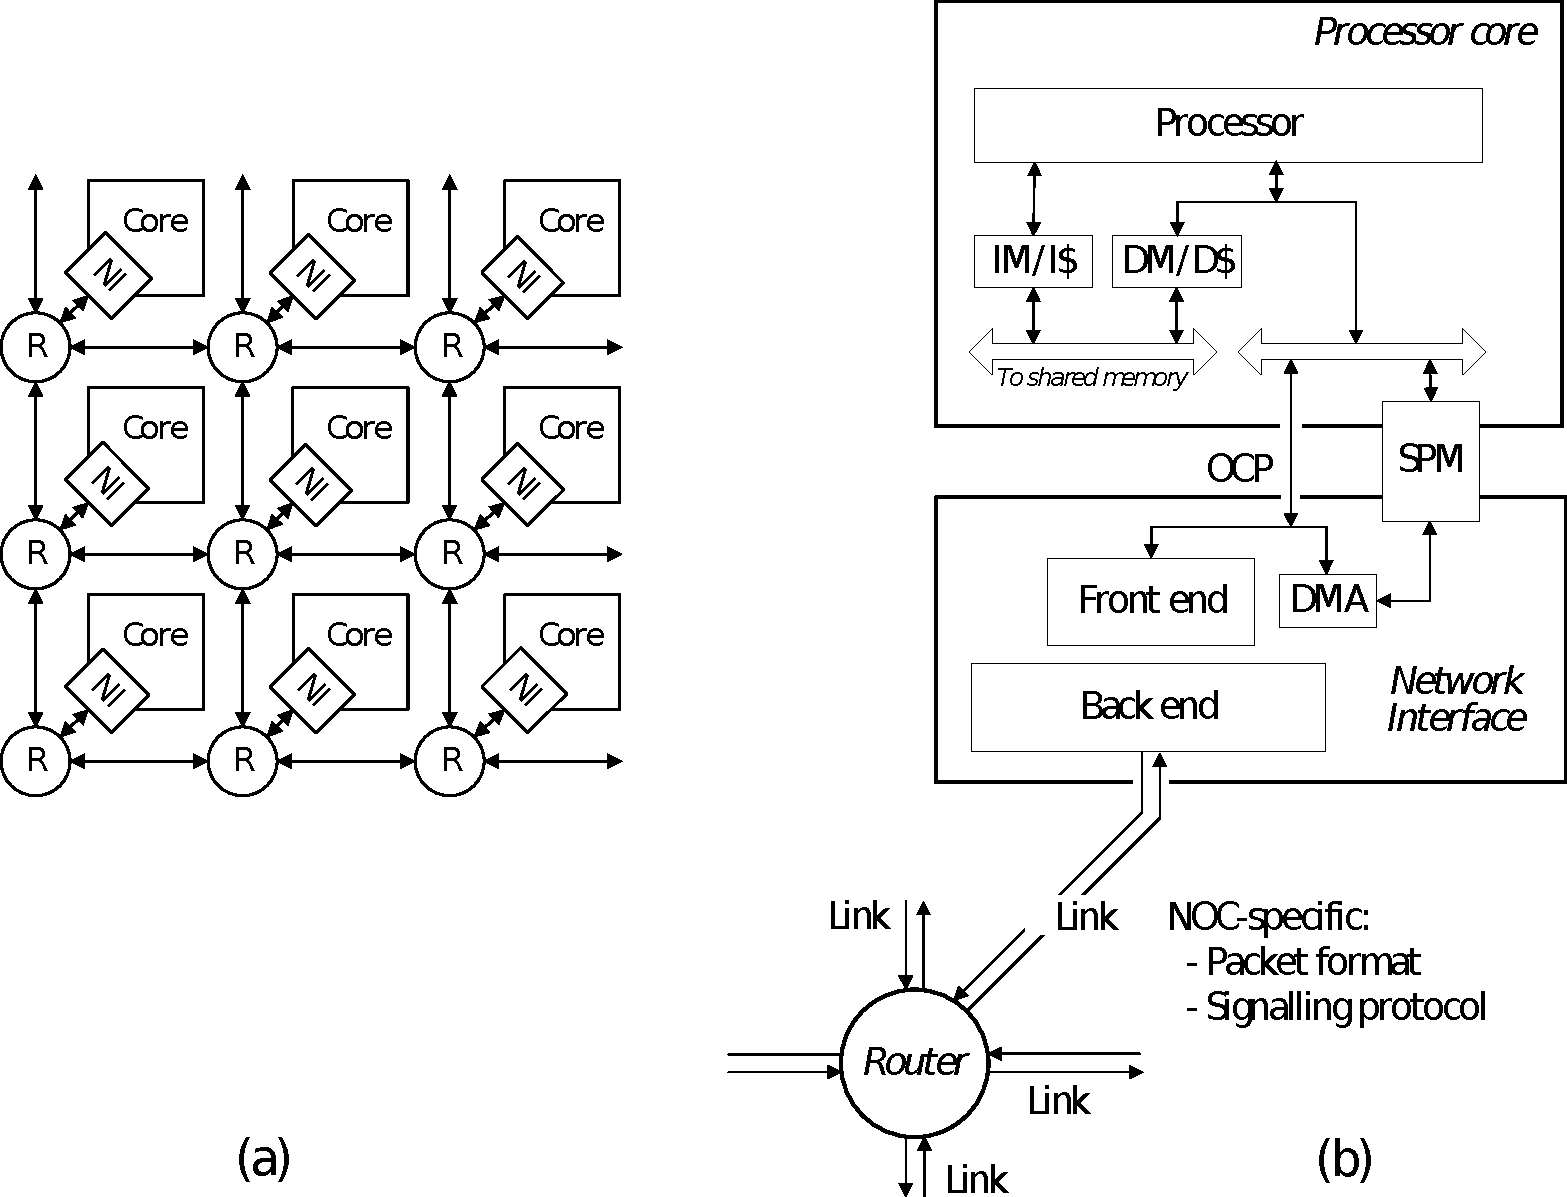
\includegraphics[scale=0.5]{fig/argo.pdf}
\caption{The architecture of a single Argo tile.}
\label{fig:diag}
\end{figure}

The communication that goes through the network is controlled by the TDM schedule.
A direct memory access (DMA) that is placed in the NI, as seen in Figure~\ref{fig:diag}(b),
is enforcing the TDM schedule.
To enable full utilization of the static TDM schedule,
Argo has a DMA channel per communication channel. 
The DMA is setup by the processor core to initiate a message send.
DMAs are creating a direct
channel from the local memory of the processor, i.e. the local scratchpad memory (SPM)
to the network. Details of the architecture and implementation of the NI can be found in \cite{tdmna}.
More details on the router design and the timing characteristics of the NOC can be found in
\cite{noc-elasticity}.



%\chapter{Static time division multiplexing scheduler}
\section{Static Time Division Multiplexing Scheduler}
\label{sec:poseidon}
The TDM scheduler used to generate schedules for Argo is called Poseidon.
The source of Poseidon is placed at \url{https://github.com/t-crest/poseidon.git}.
The performance of Poseidon is desrcibed in \cite{tcrest:poseidon}.% Technical report on poseidon

Poseidon takes an XML file as input descriping the platform and the required communication pattern.
The platform and communication tags can be given in two different XML files or on one.
When the platform is generated from the Aegean platform generator, the input files for the scheduler are also generated.

For the time beeing the scheduler is limited to schedule one package per communication channel in each period.
This limitation is due to a limitation in the current hardware, not a limitation in the scheduler it self.
When multiple packages per communication channel are supported the limitation can be removed by commenting out (in t-crest/poseidon/src/parser.cpp) the lines:

\begin{verbatim}
warn_if(bw != 1,"Bandwidth different from 1 is not supported by Argo, Bandwidth set to 1.");
if (bw != 1) { bw = 1;  }
\end{verbatim}

%\subsection{Input format}

%\subsection{Output format}

%\subsection{Conversion to C}





%\chapter{Memory address space and interface}
\section{Memory address space and interface}
\label{sec:mem}

The network interface (NI) of Argo has 2 OCP \cite{ocp:spec} interfaces. One is connected to the SPM
to access data, and the other is connected to the processor core for configuration purposes.

The SPM, the DMA and the slot table of each processor are mapped in the local address space.
They can be accessed by the processor through specific load and store instructions.

The UART and LEDS are also mapped in the local address space and can be accessed only by the master core
at the specific addresses.

\subsection{Local Address Space}

\begin{description}
\item[UART\_STATUS]      0xF0000800
\item[UART\_DATA]        0xF0000804
\item[LEDS]              0xF0000900
\item[NOC\_DMA\_BASE]    0xE0000000
\item[NOC\_DMA\_P\_BASE] 0xE1000000
\item[NOC\_ST\_BASE]     0xE2000000
\item[NOC\_SPM\_BASE]    0xE8000000
\item[NOC\_VALID\_BIT]   0x08000
\item[NOC\_DONE\_BIT]    0x04000
\end{description}


%\chapter{Build Instructions}
\section{Build Instructions}

%In the following we present the Patmos build instructions on a Linux/Ubuntu
%system.\footnote{I used the 32-bit version of Ubuntu to simplify the Quartus installation.}
%Patmos and the compiler have also been successfully installed on a Mac OSX
%system. The support of Windows is marginal, or basically not existent.
In the following we present the build instructions on a Linux/Ubuntu system,
for a 2x2 Aegean platform. The default hardware platform includes 4 Patmos processors 
connected by the Argo NOC and memory arbiter giving access to the shared memory.


\subsection{Patmos and Compiler Build Instructions}

Information on how to build a Patmos processor and how to run the compiler and some application examples
can be found in \cite{patmos-handbook}. 


The platform can be checked out from GitHub as part of the T-CREST project.
The T-CREST project will live in \code{\$HOME/t-crest} and the Aegean platform with Argo NOC
can be checked out and build with the same commands as for Patmos and the compiler.%, as follows:

%\begin{verbatim}
%mkdir ~/t-crest
%cd ~/t-crest
%git clone https://github.com/t-crest/patmos-misc.git misc
%./misc/build.sh
%\end{verbatim}


Several packages and tools need to be installed and setup. The list of packages 
and detailed setup instructions can be found in \cite{patmos-handbook}.
Additianally, \cite{patmos-handbook} describes a simpe Hello world application 
to be run either by simulation or on FPGA board, for a single Patmos processor.


%\section{Setup On Ubuntu 13.04}
%
%After a plain Ubuntu installation several packages need to be installed.
%The following apt-get lists the packages that need to be
%installed:\footnote{Some packages might be available in newer version
%when reading this document.}
%
%\begin{verbatim}
%sudo apt-get install git openjdk-7-jdk gitk cmake make g++ texinfo flex bison \
%  subversion libelf-dev graphviz libboost-dev libboost-program-options-dev ruby1.9.1 \
%  ruby1.9.1-dev python zlib1g-dev gtkwave gtkterm
%\end{verbatim}
%
%For the Quartus setup it is best to change the default shall to \code{/bin/bash}:
%
%\begin{verbatim}
%sudo rm /bin/sh
%sudo ln -s /bin/bash /bin/sh
%\end{verbatim}
%
%\subsection{Compiler and Patmos}
%
%We assume that the T-CREST project will live in \code{\$HOME/t-crest}.
%Patmos and the compiler can be checked out from GitHub and built as follows:
%
%\begin{verbatim}
%mkdir ~/t-crest
%cd ~/t-crest
%git clone https://github.com/t-crest/patmos-misc.git misc
%./misc/build.sh
%\end{verbatim}
%
%For developers with push permission generate an ssh key and upload
%it at GitHub (see \url{https://help.github.com/articles/generating-ssh-keys}
%for detailed instructions).
%The ssh based clone string for write access is then:
%
%\begin{verbatim}
%git clone git@github.com:t-crest/patmos-misc.git misc
%./misc/build.sh
%\end{verbatim}
%
%This will checkout several other repositories (the compiler, library,
%the Patmos source, and benchmarks) and
%build the compiler, the Patmos simulator, and the test benches.
%Therefore, take a cup of coffee and find some nice reading.
%After building the compiler add the path
%to the compiler executables into your \code{.profile}:
%\footnote{The path needs to be absolute. LLVM cannot handle
%a path relative to the home folder \textasciitilde{}, e.g., \code{\textasciitilde{}/t-crest/local/bin}.}
%
%\begin{verbatim}
%export PATH=$PATH:$HOME/t-crest/local/bin
%\end{verbatim}
%
%A complete logout from Ubuntu is needed to take effect (just closing
%a terminal window is not enough).
%
%You can test your installation by checking if the compiler is available:
%
%\begin{verbatim}
%patmos-clang
%\end{verbatim}
%
%For correct correct signing of your changes set the username and
%email in git with:
%
%\begin{verbatim}
%git config --global user.name "Joe Someone"
%git config --global user.email "joe.someone@domain.com"
%\end{verbatim}
%
%\subsection{Quartus}
%
%Download the free web edition of Quartus from Altera. The Linux version is
%installed as follows:\footnote{\url{http://www.altera.com/literature/manual/quartus_install.pdf}}
%
%\begin{verbatim}
%tar xvf Quartus-web-xxx.tar
%\end{verbatim}
%
%The software installation is started with a plain \code{setup.sh}.\footnote{Or \code{bash steup.sh}}
%Then add the bin directory of Quartus to your \$PATH.
%%
%For  the USB Blaster following additional steps are needed:
%
%\begin{verbatim}
%# Add user to dialout group for the serial port access
%sudo usermod -a -G dialout user
%
%# Add permissions to access the Altera USB Blaster
%sudo su -
%echo "SUBSYSTEM==\"usb\", DRIVER==\"usb\", ATTR{idVendor}==\"09fb\", \
%ATTR{idProduct}==\"6001\", MODE=\"0666\"" > /etc/udev/rules.d/51-usbblaster.rules
%
%udevadm control --reload-rules
%\end{verbatim}
%
%Quartus~13.1 drops the support of Cyclone~II devices. Therefore, the
%(phased out) Altera DE2-70 board is not supported anymore. Version 13.0 supports Cyclone~II\
%till Cyclone~V devices and might be the best option at the moment.
%
%\section{Setup On Mac OS X}
%
%Several tools are needed, best installed with MacPorts. For Patmos simulator and assembler:
%\code{boost}, \code{libelf}.
%For simulation with ModelSim: \code{wine}
%For Aegean: python33, py33-lxml. Make a link from python3 to python3.3 as this is the way it is invoked.
%\todo{Alex suggested a way to avoid this by querying how to invoke python.}
%
%\section{Hello World}
%
%We can start with the standard, harmless looking Hello
%World:\footnote{This example code is not part of the distribution, but
%can be put at any directory.}
%
%\begin{verbatim}
%main() {
%    printf("Hello Patmos!\n");
%}
%\end{verbatim}
%
%With the compiler installed it can be compiled to a Patmos executable
%and run with the simulator as follows:
%
%\begin{verbatim}
%patmos-clang hello.c
%pasim a.out
%\end{verbatim}
%
%However, this innocent examples is quiet challenging for an embedded system:
%It needs a C compiler, an implementation of the standard C library, printf
%itself is a challenging function, the generated ELF file needs to be understood
%by a tool and the individual sections downloaded, and finally a terminal (often
%a serial line) needs to be available on the target, and your test PC needs to
%have a serial line as well and a terminal program needs to run.
%
%Therefore, we might start from a minimal assembler program and execute
%that in the simulator and emulator. From that base we can build up too
%a multi-core version of Patmos that executes in an FPGA and bootstraps
%with programs loaded via a serial port.
%
%
%\section{Building Patmos}
%
%The whole build process of Patmos,%
%\footnote{Get the source from GitHub with: \code{git clone git@github.com:t-crest/patmos}}
%applications in assembler
%and in C, configuration of the FPGA, and downloading an application
%is \code{Makefile} based. The build of Patmos is within the patmos folder,
%therefore, the following descriptions assumes you have changed to:
%
%\begin{verbatim}
%    t-crest/patmos
%\end{verbatim}
%
%
%The complete design flow (including the LLVM
%based C compiler) can execute in a Linux machine. The flow without
%the C compiler should be able to execute in a Windows/Cygwin environment.
%Under Mac OS X all tools, except Quartus, are working (ModelSim under
%wine). For FPGA synthesis and configuration Windows XP within a VMWare
%virtual machine is a possible solution.
%
%On a Linux box with the installed LLVM compiler and Quartus in your PATH,
%the complete build processes for a Hello World is as follows:
%
%\begin{verbatim}
%make BOOTAPP=bootable-bootloader APP=hello_puts \
%   tools comp gen synth config download
%\end{verbatim}
%
%However, this involves quite many steps. Therefore, we suggest doing some \emph{manual}
%buildup to explore the full build process and the possibilities.
%
%As a start we build some tools (e.g., the assembler, simulator, file conversion
%utility, and the boot loader). This has to be done once only.
%
%\begin{verbatim}
%make tools
%\end{verbatim}
%
%\subsection{A Few Assembler Instructions}
%
%We start with a very small assembler program that moves a few values into registers
%(see \code{asm/basic.s}). With following make command the program is assembled
%and executed in the software simulator of Patmos.
%
%\begin{verbatim}
%make swsim BOOTAPP=basic
%\end{verbatim}
%
%The simulator options are set to write out the register contents after each instruction.
%The emulator (the Chisel based simulator) can execute the same program
%with following command:
%
%\begin{verbatim}
%make hwsim BOOTAPP=basic
%\end{verbatim}
%
%This command assembles the application, executes the Chisel based hardware
%construction during which the program is used to initialize the on-chip ROM,
%generates a C++ based emulator, compiles that emulator, and executes it.
%The emulator show the register content after each instruction.
%
%Those two Patmos simulations, the software simulator and the Chisel based emulator,
%are used for a co-simulation based test. In this co-simulation all available assembler
%programs are executed in both simulations and the register out put is compared.
%The test can be started with:
%
%\begin{verbatim}
%make test
%\end{verbatim}
%
%
%\todo{ModelSim simulation}
%
%\subsection{We Can Blink in Assembler}
%
%\todo{write}
%
%\subsection{A C Based Blinking LED}
%
%As a first real example we build the embedded version of Hello World, the
%blinking LED, from a C program. You can find the C source in \code{c/blinking.c}.
%
%\begin{verbatim}
%make BOOTAPP=bootable-blinking comp gen synth config
%\end{verbatim}
%
%Additionally to blinking an LED this program also writes alternating `0' and `1'
%to the serial port. Connect the FPGA board to your serial port,
%open a terminal of your choice (e.g., \code{gtkterm}), connect to the serial port,
%set the baud rate to 115200, no parity, and no handshaking.
%You should see alternating `0' and `1' sent out synchronous to the blinking.
%
%Note that the program name (\code{blink}) is prefixed by \code{bootable-}.
%The marker selects the right compiler settings for a program that ends up in
%the Patmos on-chip ROM. As the on-chip memory is limited, only tiny programs
%are supported in this execution mode.
%
%Figure~\ref{fig:blink} shows the code for the embedded Hello World
%C program. Two constants (0xF0000900 and 0xF0000804) are the addresses
%of the IO devices LED and serial port. IO devices connected to Patmos are
%connected to the local, uncached memory area. This is the same memory
%area where data SPM and NoC SPM are connected. Therefore, to access them
%one needs to use the local load/store instructions. With the attribute \code{\_SPM}
%the compiler is instructed to emit the correct load and store instructions.
%
%\begin{figure}
%\begin{verbatim}
%/*
%    This is a minimal C program executed on the FPGA version of Patmos.
%    An embedded Hello World program: a blinking LED.
%
%    Additional to the blinking LED we write to the UART '0' and '1' (if available).
%
%    Author: Martin Schoeberl
%    Copyright: DTU, BSD License
%*/
%
%#include <machine/spm.h>
%
%int main() {
%
%    volatile _SPM int *led_ptr = (volatile _SPM int *) 0xF0000900;
%    volatile _SPM int *uart_ptr = (volatile _SPM int *) 0xF0000804;
%    int i, j;
%
%    for (;;) {
%        *uart_ptr = '1';
%        for (i=2000; i!=0; --i)
%            for (j=2000; j!=0; --j)
%                *led_ptr = 1;
%
%
%        *uart_ptr = '0';
%        for (i=2000; i!=0; --i)
%            for (j=2000; j!=0; --j)
%                *led_ptr = 0;
%
%    }
%}\end{verbatim}
%\caption{A blinking LED}
%\label{fig:blink}
%\end{figure}
%
%\martin{I'm still a little bit confused when to use the APP and the BOOTAPP
%thing.}
%
%\martin{TODO: we need to streamline the make process a little bit.
%The targets might be a little bit confusing. Patmos is compiled two times.}
%
%
%\subsection{Make Targets}
%
%A list of the most important make targets:
%
%\begin{description}
%\item[tools] build of all tools, including the Patmos software simulator
%\item[asm] assemble source (from folder \code{asm})
%\item[swsim] execute the Patmos emulator
%\item[hwsim] execute the Patmos emulator
%\item[emulator] build the Chisel based C++ emulator
%\item[comp] compile a C program as loadable ELF binary
%\item[bootcomp] compile a C program as a bootable image
%\item[gen] generate the Verilog code
%\item[synth] synthesize for an FPGA
%\item[config] configure the FPGA
%\item[download] download an elf file into the main memory via the Patmos bootloader
%\item[test] run all assembler tests 
%\end{description}
%
%The name of an application that can execute from the on-chip ROM is set
%with the BOOTAPP variable.
%
%\subsection{Download of ELF Files}
%
%On a Linux box with the installed LLVM compiler and Quartus in your PATH,
%the complete build processes for the Hello World is as follows:
%
%% make BOOTAPP=bootable-bootloader APP=hello_puts tools synth comp config download
%\begin{verbatim}
%make BOOTAPP=bootable-bootloader APP=hello_puts \
%   tools comp gen synth config download
%\end{verbatim}
%
%You should see the download information and then the greeting from Patmos:
%
%\begin{verbatim}
%/home/martin/t-crest/patmos/install/bin/patserdow -v /dev/ttyUSB0 /home/martin/t-crest/patmos/tmp/hello_puts.elf
%Port opened: true
%Params set: true
%Elf version is '1':true
%CPU type is:48875
%Instruction width is 32 bits:true
%Is Big Endian:true
%File is of type exe:true
%Entry point:131076
%
%[++++++++++] 49778/49778 bytes
%Hello, World!
%
%EXIT 0
%\end{verbatim}
%
%The \code{Makefile} use following variables to configure the build process:
%\code{BOOTAPP} is an application that ends in the on-chip ROM. This may
%be an assembler program or a simple C program;
%most prominent the boot loader for ELF binaries.
%A C program that shall be compiled as ROM target needs to be prefixed
%with \code{bootable-}.
%\code{APP} is a C program resulting in an ELF binary that can be either
%loaded by the emulator or the boot loader when executing in an FPGA.
%% TODO: test and talk about patsim. Having a complete ELF in the FPGA
%% without the boot loader would be nice as well.
%
%\todo{Describe ELF download without building the FPGA}
%
%
%Here an example of the individual steps to build the blinking LED C
%hello world (on a different FPGA board):
%\begin{verbatim}
%make tools
%make BOOTAPP=bootable-echo bootcomp gen
%make BOOTAPP=bootable-echo QPROJ=bemicro synth
%make QPROJ=bemicro BLASTER_TYPE=Arrow-USB-Blaster config
%\end{verbatim}
%
%This split of the make commands is for demonstration. It is
%possible to merge all steps into a single make (on Linux
%systems) or two steps when using two operating
%systems (e.g., Mac OSX for compilation and Windows for synthesis).
%
%\paragraph{Emulator and elf File}
%
%The emulator can read a standard ELF file. An example how to compile
%a small C program that uses part of the standard library and executing
%it on the emulator is as follows:
%
%\begin{verbatim}
%make emulator
%make comp APP=hello_puts
%hardware/build/emulator tmp/hello_puts.elf
%\end{verbatim}
%
%\martin{Where is the make target to run the emulator with an ELF file?}
%
%\subsection{Supported FPGA Boards}
%
%At the time of this writing we have mainly focused on Altera FPGA based boards. Following boards
%are directly supported in the default build process:
%
%\begin{itemize}
%\item Altera DE2-70 (\code{altde2-70})
%\item Altera DE2-115 (\code{altde2-115})
%\item Altera/Farnell BeMicro (\code{bemicro})
%\end{itemize}
%
%The board is configured by setting the \code{BOARD} variable.
%Without changing the \code{Makefile} the default of the board (and any other build variables)
%can be overridden by providing a local \code{config.mk} that is included in the Makefile.
%
\subsubsection{Aegean}

The whole build process of a 2x2 Aegean platform,
\footnote{Get the source from GitHub with: \code{git clone git@github.com:t-crest/aegean}} 
applications %in assembler
in C, configuration of the FPGA, and downloading an application
is \code{Makefile} based. The build of the platform is done in the aegean folder,
therefore, the following descriptions assumes you have changed to:

\begin{verbatim}
	t-crest/aegean
\end{verbatim}

The default platform is 4 Patmos cores connected by Argo NOC 
and a memory arbiter connecting to main memory.
The platform is generated by command:

\begin{verbatim}
make platform
\end{verbatim}

To synthesize the platform for the Altera DE2-115 FPGA board, along with the bootloader application run:

\begin{verbatim}
make synth
\end{verbatim}

The synthesized platform is configured on the FPGA with the command:

\begin{verbatim}
make config
\end{verbatim}

The default board is the Altera DE2-115 FPGA board. The target board can be changed by
setting the \code{BOARD} variable in the above make commmands. The currently supported boards are:

\begin{itemize}
\item Altera DE2-70 (\code{altde2-70})
\item Altera DE2-115 (\code{altde2-115})
\item Altera/Farnell BeMicro (\code{bemicro})
\end{itemize}


\subsection{Applications}

Applications for the multicore platform can be developed in C code, either 
compiled with the hardware platform, embedded in the the on-chip ROM
or compiled in ELF binaries, bootable by the emulator or the bootloader on FPGA.
The application is written in C and placed under /t-crest/patmos/c.
In both cases the application is build through \code{Makefile}
using the following variables:

\begin{itemize}
\item \code{BOOTAPP} for the built in on-chip ROM applications.
\item \code{APP} for the ELF binary applications to be executed through bootloader.
\end{itemize}

%The \code{Makefile} use following variables to configure the build process:
%\code{BOOTAPP} is an application that ends in the on-chip ROM. This may
%be an assembler program or a simple C program;
%most prominent the boot loader for ELF binaries.
%A C program that shall be compiled as ROM target needs to be prefixed
%with \code{bootable-}.
%\code{APP} is a C program resulting in an ELF binary that can be either
%loaded by the emulator or the boot loader when executing in an FPGA.
%% TODO: test and talk about patsim. Having a complete ELF in the FPGA
%% without the boot loader would be nice as well.
%

\subsection{Applications and download of ELF files}

An application executed in the multicore platform can be compiled in an ELF file and downloaded on the FPGA.
%The application should be written in C and placed under /t-crest/patmos/c. 
The compilation and downloading
is make-based and is done in folder /t-crest/patmos/ with the following make commands:

\begin{verbatim}
make APP=<app_name> comp
make APP=<app_name> download
\end{verbatim}


%\section{ModelSim License}
%In the case that you have a DTU Compute login you can access the license servers from outside the DTU network by setting up an SSH tunnel.
%An example of how such a tunnel can be set up follows, you need to insert you own username.
%
%\begin{verbatim}
%ssh -L 1717:angel2:1717 -L 1718:angel2:1718 ${USERNAME}@sshlogin.compute.dtu.dk
%\end{verbatim}
%
%When the SSH tunnel is setup the LM\_LICENSE\_FILE needs to be set to:
%\begin{verbatim}
%LM_LICENSE_FILE=1717@localhost
%\end{verbatim}
%
%This way of setting up an SSH tunnel might also work for other institutions.
%
%% MS: there needs to be more content to have a chapter on the compiler.
%
%\chapter{The Patmos Compiler}
%\label{sec:compiler}
%
%The LLVM compiler has been adapted to emit code for the Patmos ISA
%and support the special features, e.g., the stack cache~\cite{Seus13:compiler}.
%
%\martin{Daniel and Stefan shall add here an overview of the compiler and
%some words on source organization. But let's start with some notes.}
%
%The compiler and libraries can be built with \code{misc/build.sh}.
%This script also contains the default options, which should work on a
%standard Linux machine out of the box. Options can be overwritten by
%entries in a personal \code{misc/build.cfg}. The file {misc/build.dist.cfg}
%is just an example configuration file, generated from build.sh, and ignored
%by the build process.

%\chapter{Application Programming Guide}
\section{Application Programming Guide}
\label{sec:apg}

\subsection{Application Programming Interface}

Library libnoc is providing an application programming interface. A number of functions and variables are provided through libnoc library. libnoc offers two kinds of functionality, the first is to initialize the network interface (NI) and the second is the setup DMA transfers for sending messages to other processing cores. 

The variables defined in libnoc:
\begin{description}
\item[NOC\_CORES] The number of cores on the platform. 
\item[NOC\_TABLES] The number of tables for Noc configuration. 
\item[NOC\_TIMESLOTS] The number of timeslots in the schedule. 
\item[NOC\_DMAS]	The number of DMAs in the configuration. 
\item[noc\_init\_array] The array for initialization data. 
\item[NOC\_MASTER] The master core, which governs booting and startup synchronization. 
\end{description}


The functions defined in libnoc:
\begin{description}
\item [noc\_configure] Configure network interface according to initialization information in noc\_init\_array.
\item [noc\_init] Configure network-on-chip and synchronize all cores. 
\item [noc\_dma] Starts a NoC transfer. 
\item [noc\_send] Transfer data via the NoC. 
\end{description}

The defines in libnoc:
\begin{description}
\item [NOC\_INIT] Define this before including noc.h to force the use of noc\_init as constructor. NOC\_INIT does not need to be defined if any functions from libnoc are used.
\item [NOC\_VALID\_BIT] The flag to mark a DMA entry as valid.
\item [NOC\_DONE\_BIT] The flag to mark a DMA entry as done.
\item [NOC\_DMA\_BASE] The base address for DMA entries.
\item [NOC\_DMA\_P\_BASE] The base address for DMA routing information.
\item [NOC\_ST\_BASE] The base address for the slot table.
\item [NOC\_SPM\_BASE] The base address of the communication SPM.
\end{description}

\subsection{Hello World Multicore}

To demonstrate the use of Argo, a multicore Hello World application \textit{hello\_sum.c} is placed in /patmos/c.
The application is written in C and can be compiled and downloaded on the FPGA board.

\subsubsection{Compile and Run}
For any application to be compiled and run, it needs to be placed in /patmos/c. To compile and download \textit{hello\_sum} application on the board, the following make commands are used:

\begin{verbatim}
make APP=hello_sum comp
make APP=hello_sum download
\end{verbatim}

\subsubsection{SPM Access}
To develop an application that runs on T-CREST platform, memory access and 
communication should be handled explicitely by the programmer. Argo NOC is initialized automatically 
through Aegean platform but the communication of data should be handled by the application programmer.
Specifically, in \textit{hello\_sum} application, a round trip hello message is sent from the master
passing through all the cores. Each core is adding its id to the sum of the id and 
eventually the master will receive the sum of all core ids. To send data from one core to another 
the data should be explicitely placed in the local SPM of the core. Pointers to access SPM space are defined as:

\begin{lstlisting}
volatile _SPM <type> *<name>
\end{lstlisting}

The copying of the message should be done manually, copying one-by-one character or integer.
Copying of strings through string.h is not available. 

%Listing~\ref{lst:hello_master} shows the code executed in the master core.
%The code for the explicit copying the data to the SPM space, the sending of message,

\subsubsection{Sending}
A message is sent using function noc\_send():

\begin{lstlisting}
void noc_send (int rcv_id, volatile void _SPM *dst, volatile void _SPM *src, size_t size)
\end{lstlisting}

The function returns when the DMA transmitting the message is setup. \code{rcv\_id}
is the ID of the receiving core, \code{dst} the write address
in the destination SPM, \code{src} the read address
in the source SPM and \code{size} the size of the message to be transfered in bytes.

\begin{lstlisting}[float,caption={A 2x2 Hello World application: Master.\label{lst:hello_master}}]
volatile _SPM char *spm_base = (volatile _SPM char *) NOC_SPM_BASE;
volatile _SPM char *spm_slave = spm_base+NOC_CORES*16;

// message to be send
const char *msg_snd = "Hello slaves sum_id:0";
char msg_rcv[22];

// put message to spm
int i;
for (i = 0; i < 21; i++) {
	*(spm_base+i) = *(msg+i);
}

// send message
noc_send(1, spm_slave, spm_base, 21); //21 bytes

puts("MASTER: message sent: ");
puts(msg_snd);

// wait and poll
while(*(spm_slave+20) == 0) {;}

// received message
puts("MASTER: message received:");
// copy message to static location and print
for (i = 0; i < 21; i++) {
	*(msg_rcv+i) = *(spm_slave+i);
}
*(msg_rcv+i) = '\0';
puts(msg_rcv);

\end{lstlisting}


The explicit copying of data to the SPM space and the sending of message appears 
in Listing~\ref{lst:hello_master}. Listing~\ref{lst:hello_master}
shows the code executed in the master core.

\subsubsection{Receiving}
Currently, libnoc library does not support a receive message function,
therefore a receiver needs to wait and poll in order to know when the data has arrived.
To do so, specified addresses where the data are expected to arrive are used by the
application and the receiving application is polling this address to
know if the data have arrived or not. 
Since data is transmitted in packets, to safely consider the reception of the entire message
completed, the polling should be done on the last unit of data (char/ int/...) of the message sent.
Listing \ref{lst:hello_multi} shows the code executed in the slave cores.
The code for the allocation of memory in the SPM, the polling and the sending of message 
appears in Listing \ref{lst:hello_multi}. In the code, \begin{verbatim} spm_slave \end{verbatim}
is the starting addres where the data is expected in the slave cores. 
\begin{verbatim} spm_slave + 20 \end{verbatim} is the last char expected in the destination.
Thus, when the last char arrives it is safe to assume that the entire message has arrived.


\begin{lstlisting}[float,caption={A 2x2 Hello World application: Slave.\label{lst:hello_multi}}]
volatile _SPM char *spm_base = (volatile _SPM char *) NOC_SPM_BASE;
volatile _SPM char *spm_slave = spm_base + NOC_CORES*16;

// wait and poll until message arrives
while(*(spm_slave + 20) == 0) {;}

// PROCESS : add ID to sum_id
*(spm_slave+20) = *(spm_slave+20) + CORE_ID;

// send to next slave
int rcv_id = (CORE_ID==3)? 0 : CORE_ID+1;
noc_send(rcv_id, spm_slave, spm_slave, 21);

\end{lstlisting}

\subsubsection{Printing}
To print a message, functions \code{puts} and \code{printf} can be used. Data can be print only
by the master core and only if it is placed in the static memory of the program. Therefore,
a data value that is placed in the SPM should be copied in a static variable 
and then print through \code{puts} or \code{printf}. Listing~\ref{lst:hello_master}
shows how to print a static string and a message received in SPM through NOC.


%\chapter{Pending Changes}
%\section{Pending Changes}
%
%This is a live and temporary section that lists pending changes of Argo.
%
%Currently we have following proposals for a change:
%
%\begin{itemize}
%\item DMA read
%\item Generate an interrupt when a complete DMA transfer has been received. 
%\end{itemize}

% % % % % % % % % % % % % % % % % % % % % % % % % % % % % % % % % % % % % % % %
%\chapter{Potential Extensions}
%\section{Potential Extensions}
%\label{chap:ext}
%Ideas for extensions can be added in this chapter.



\bibliographystyle{abbrv}
% MS noc.bib is missing
\bibliography{argobib}

\end{document}

\appendix


\end{document}
